
\documentclass[12pt,a4paper]{report}
\usepackage{fontspec}
\setmainfont{Times New Roman}
\setmonofont{Courier New}
\usepackage[top=2.5cm,bottom=2.5cm,left=3cm,right=2cm]{geometry}
\usepackage{amsmath,amssymb}
\usepackage{graphicx}
\usepackage{booktabs,tabularx,array}
\usepackage{float}
\usepackage{xcolor}
\usepackage{tikz}
\usetikzlibrary{arrows.meta,positioning,shapes.geometric}
\usepackage{hyperref}
\usepackage{fancyhdr}
\usepackage{titlesec}
\usepackage{caption}
\usepackage{enumitem}
\usepackage{fvextra}

\definecolor{reportblue}{RGB}{0,45,145}
\definecolor{softblue}{RGB}{237,244,251}
\hypersetup{colorlinks=true,linkcolor=reportblue,citecolor=reportblue,
  urlcolor=reportblue,pdftitle={Bao cao AI Agents va Q-learning},
  pdfauthor={Phan Van Khoi}}
\renewcommand{\chaptername}{Phần}
\renewcommand{\contentsname}{Mục lục}
\renewcommand{\figurename}{Hình}
\renewcommand{\tablename}{Bảng}
\renewcommand{\bibname}{Tài liệu tham khảo}
\titleformat{\chapter}[display]
  {\normalfont\bfseries\color{reportblue}}
  {\filleft\Large\chaptername\ \thechapter}{1ex}
  {\titlerule\vspace{1ex}\filright\LARGE}
  [\vspace{1ex}\titlerule]
\titleformat{\section}{\normalfont\large\bfseries\color{reportblue}}{\thesection}{0.7em}{}
\setlength{\parindent}{1.1cm}
\setlength{\parskip}{0.28em}
\linespread{1.16}
\setlist[itemize]{leftmargin=1.8em,itemsep=0.18em,topsep=0.25em}
\setlist[enumerate]{leftmargin=1.8em,itemsep=0.18em,topsep=0.25em}
\captionsetup{font=small,labelfont=bf}
\DefineVerbatimEnvironment{Code}{Verbatim}{fontsize=\scriptsize,frame=single,
  breaklines=true,breakanywhere=true,baselinestretch=1.0}
\DefineVerbatimEnvironment{Output}{Verbatim}{fontsize=\small,frame=single,
  breaklines=true,breakanywhere=true}
\pagestyle{fancy}
\fancyhf{}
\fancyhead[R]{\small\itshape Agent 01: AI Agents và Q-learning}
\fancyfoot[C]{\thepage}
\setlength{\headheight}{15pt}

\begin{document}
\hypersetup{pageanchor=false}
\begin{titlepage}
\thispagestyle{empty}
\begin{center}
\vspace*{0.7cm}
{\bfseries\fontsize{16}{20}\selectfont HỌC VIỆN CÔNG NGHỆ BƯU CHÍNH VIỄN THÔNG}\\[0.15cm]
{\bfseries\fontsize{15}{19}\selectfont KHOA CÔNG NGHỆ THÔNG TIN 1}\\[0.3cm]
\rule{5cm}{0.5pt}
\vspace{2.2cm}

{\bfseries\fontsize{18}{24}\selectfont BÁO CÁO MÔN HỌC}\\[0.35cm]
{\bfseries\fontsize{17}{23}\selectfont PHÁT TRIỂN CÁC HỆ THỐNG THÔNG MINH}\\[0.7cm]
{\bfseries\color{reportblue}\fontsize{22}{28}\selectfont AI AGENTS VÀ HỌC TĂNG CƯỜNG}\\[0.3cm]
{\bfseries\fontsize{16}{21}\selectfont Tổng quan và thực hành Q-learning giải mê cung}

\vspace{2.0cm}
\begin{tabular}{>{\bfseries}p{4.1cm}p{6.5cm}}
Họ tên: & Phan Văn Khôi \\
Mã sinh viên: & B23DCCN447 \\
Lớp: & D23CTPM01-B \\
Giảng viên: & PGS. TS. Trần Đình Quế \\
\end{tabular}
\vfill
{\bfseries\fontsize{14}{18}\selectfont Hà Nội -- 2026}
\end{center}
\end{titlepage}
\hypersetup{pageanchor=true}
\pagenumbering{roman}
\tableofcontents
\clearpage
\pagenumbering{arabic}

\chapter{Tổng quan về AI Agents}
\label{chap:agents}

\section{Khái niệm, mức tự chủ và phạm vi}
AI agent là một hệ thống phần mềm được giao mục tiêu, có khả năng chọn và thực hiện
hành động để hoàn thành công việc thay mặt người dùng hoặc một hệ thống khác. Google
Cloud nhấn mạnh năng lực suy luận, lập kế hoạch, ghi nhớ và thích ứng; IBM đặt trọng tâm
vào việc agent tự tổ chức quy trình và gọi công cụ; McKinsey xem agent là thành phần có
quyền hành động, có thể được phối hợp thành hệ thống xử lý quy trình phức tạp
\cite{google,ibm,mckinsey}. Ba cách diễn đạt cùng chỉ ra hai điều kiện cốt lõi: agent theo
đuổi một mục tiêu và có thể tác động đến môi trường để đạt mục tiêu đó.

Mức tự chủ không phải thuộc tính có hoặc không. Một agent có thể chỉ đề xuất bước
tiếp theo, thực hiện tác vụ sau khi người dùng duyệt, hoặc tự xử lý nhiều bước trong
giới hạn được cấp. Giới hạn ấy do người thiết kế, đơn vị triển khai và người dùng đặt ra;
IBM nhấn mạnh agent vẫn cần mục tiêu cùng quy tắc do con người xác định
\cite{ibm}. Vì vậy, "tự chủ" không có nghĩa là không cần kiểm soát.

Theo Google Cloud, \emph{assistant} thường cộng tác trực tiếp với người dùng qua từng
bước, còn \emph{bot} truyền thống chủ yếu phản hồi theo quy tắc hoặc kích hoạt định
sẵn. Agent có thể chủ động hơn, xử lý nhiều hành động liên tiếp và điều chỉnh kế hoạch
theo phản hồi \cite{google}. Ranh giới thực tế vẫn phụ thuộc sản phẩm: một assistant có
thể được trao công cụ và quyền hành động để vận hành như agent.

AI agent cũng không đồng nhất với mô hình ngôn ngữ lớn (LLM). LLM có thể hiểu và tạo
ngôn ngữ, nhưng agent còn cần mục tiêu, trạng thái, quy trình điều phối và kênh hành
động. McKinsey lưu ý một hệ thống có thể dùng LLM để giao tiếp nhưng dùng mô hình
chuyên biệt cho quyết định kỹ thuật, ví dụ một chức năng an toàn trên xe
\cite{mckinsey}. Agent trong notebook Q-learning ở Phần 2 là ví dụ không dùng LLM.

\section{Thành phần của một agent}
Một kiến trúc agent thường có các thành phần sau. \textbf{Mục tiêu và ràng buộc} xác
định thành công là gì, quyền nào được dùng và khi nào phải dừng. \textbf{Bộ xử lý trung
tâm} có thể là LLM, mô hình chuyên biệt hoặc tập luật; nó diễn giải tình huống và chọn
bước tiếp theo. \textbf{Bộ nhớ} lưu ngữ cảnh tác vụ, thông tin trước đó hoặc kinh nghiệm
để không phải bắt đầu lại sau mỗi bước. \textbf{Công cụ} cung cấp khả năng tìm kiếm,
truy cập dữ liệu, gọi API, sửa tệp hoặc thao tác trên hệ thống bên ngoài. Google Cloud
liệt kê model, memory, tools và mô tả vai trò agent như các yếu tố vận hành quan trọng
\cite{google}.

\begin{figure}[H]
\centering
\begin{tikzpicture}[node distance=7mm and 9mm,>=Stealth,
  box/.style={draw=reportblue,rounded corners,fill=softblue,
  align=center,minimum height=9mm,text width=3.2cm,font=\small}]
\node[box] (goal) {Mục tiêu và giới hạn};
\node[box,right=of goal] (agent) {Agent: quan sát, suy luận, lập kế hoạch};
\node[box,right=of agent] (tool) {Công cụ và môi trường};
\draw[->,thick] (goal) -- (agent);
\draw[->,thick] (agent) -- node[above,font=\scriptsize]{hành động} (tool);
\draw[->,thick] (tool.south) -- ++(0,-0.45) -| node[pos=.25,below,font=\scriptsize]{kết quả, phản hồi} (agent.south);
\end{tikzpicture}
\caption{Vòng tương tác khái quát của AI agent, tổng hợp từ ba nguồn.}
\end{figure}

Bộ nhớ có thể phục vụ ngữ cảnh ngắn hạn của nhiệm vụ hoặc ghi lại lịch sử dài hạn;
chất lượng của nó phụ thuộc dữ liệu lưu và cách truy xuất, chứ không tự động đảm bảo
agent "học" theo nghĩa cập nhật trọng số mô hình. Một agent có thể cải thiện câu trả
lời nhờ nhớ phản hồi mà không trải qua huấn luyện lại. Công cụ cũng làm tăng năng lực
lẫn rủi ro: quyền ghi dữ liệu hoặc gửi thông điệp mở rộng phạm vi sai sót so với một
hệ chỉ tạo văn bản. Bởi vậy, cấu trúc kỹ thuật phải đi cùng phân quyền và kiểm tra
kết quả \cite{google,ibm}.

\section{Quy trình hoạt động từ mục tiêu đến hành động}
IBM mô tả ba giai đoạn: khởi tạo mục tiêu và lập kế hoạch, suy luận với công cụ, rồi
học và phản tư từ phản hồi. McKinsey mô tả một hệ thống nhận nhiệm vụ, chia việc và
thực thi, cải thiện đầu ra lặp lại nếu cần, sau đó hoàn thành hành động
\cite{ibm,mckinsey}. Có thể ghép hai góc nhìn thành một chu trình thực tế:
\begin{enumerate}
\item \textbf{Hiểu yêu cầu:} xác định kết quả cần tạo, dữ liệu đầu vào và điều kiện dừng.
\item \textbf{Lập kế hoạch:} chia mục tiêu thành các việc có thứ tự; việc đơn giản có thể bỏ qua bước lập kế hoạch tường minh.
\item \textbf{Quan sát và dùng công cụ:} lấy thông tin còn thiếu từ nguồn được phép, thực hiện hành động phù hợp.
\item \textbf{Đánh giá:} đối chiếu kết quả với mục tiêu; sửa sai, hỏi người dùng hoặc chuyển cấp khi vượt thẩm quyền.
\item \textbf{Kết thúc:} trả kết quả và ghi lại thông tin cần thiết cho lần sau.
\end{enumerate}

Google Cloud nhấn mạnh các năng lực quan sát, suy luận, hành động, lập kế hoạch, cộng
tác và tự điều chỉnh \cite{google}. Các năng lực này không nhất thiết xuất hiện với
cùng độ mạnh trong mọi sản phẩm. Chẳng hạn, agent xử lý sự kiện nền cần quan sát trạng
thái hệ thống liên tục; agent hỗ trợ viết nội dung chú trọng đối thoại và đánh giá văn
bản. Cả hai vẫn phải kiểm tra xem hành động đã tạo ra kết quả thực hay mới chỉ tạo ra
một câu trả lời có vẻ hợp lý.

Trong hệ dùng LLM, mô hình thường chọn công cụ dựa trên thông tin hiện có rồi cập
nhật ngữ cảnh sau khi nhận kết quả. IBM gọi cách lặp suy luận, hành động và quan sát
này là ReAct; bài viết cũng nêu ReWOO, nơi kế hoạch dùng công cụ được hình thành trước
khi lấy kết quả \cite{ibm}. Đây là hai cách tổ chức quá trình, không phải định nghĩa
duy nhất của AI agent. Nếu đầu ra công cụ sai hoặc thiếu, agent phải kiểm tra lại giả
định, giới hạn số lần thử và biết dừng thay vì lặp vô hạn.

\section{Tình huống minh họa: xử lý yêu cầu khách hàng}
Giả sử một khách hàng hỏi vì sao đơn hàng giao chậm và muốn đổi địa chỉ nhận. Đây
là ví dụ giả định để nối các thành phần kỹ thuật ở trên, không phải một ca triển
khai được ba nguồn đo lường. Google Cloud xếp các hệ hỗ trợ cá nhân hóa và giải
quyết yêu cầu như vậy vào nhóm agent phục vụ khách hàng; McKinsey mô tả các quy
trình có nhiều bước, có thể giao việc cho các agent chuyên biệt \cite{google,mckinsey}.

Đầu tiên, agent tiếp nhận yêu cầu và xác định hai kết quả khác nhau: giải thích
tình trạng giao hàng và thay đổi dữ liệu đơn hàng. Agent cần biết mã đơn, danh tính
người yêu cầu và quyền sửa đơn. Thông tin người dùng cung cấp trong hội thoại có
thể chưa chính xác hoặc chưa đủ, vì vậy agent tra cứu dữ liệu từ hệ quản lý đơn
hàng thay vì tự suy đoán ngày giao. Nếu công cụ không trả kết quả, câu trả lời phù
hợp là nêu giới hạn và chuyển sang bước kiểm tra khác hoặc nhờ người phụ trách.

Tiếp theo, agent đối chiếu trạng thái vận chuyển với quy định đổi địa chỉ. Nếu đơn
đã được bàn giao cho đơn vị vận chuyển, quy định có thể khác so với đơn còn ở kho.
Đây là chỗ cần công cụ dữ liệu và nguồn chính sách được cập nhật. Bộ nhớ hội thoại
giúp agent giữ mã đơn và yêu cầu trước đó trong cùng phiên, nhưng mọi kết luận về
trạng thái đơn vẫn cần căn cứ ở dữ liệu nghiệp vụ hiện hành. Agent có thể chia việc
tra trạng thái, kiểm tra quy định và soạn câu trả lời; một bước kiểm tra cuối cùng
phải ghép các kết quả thành một đề xuất nhất quán \cite{ibm,mckinsey}.

Sau khi biết đơn đủ điều kiện đổi địa chỉ, agent nên trình bày địa chỉ hiện tại,
địa chỉ mới và hệ quả có thể có, rồi xin xác nhận trước khi ghi thay đổi. Việc
"đã soạn đề xuất" khác với "đã sửa thành công". Chỉ sau khi API ghi dữ liệu phản
hồi thành công và một lần đọc lại cho thấy trạng thái mới, agent mới thông báo đã
hoàn tất. Nếu thao tác lỗi giữa chừng, nhật ký phải cho biết bước nào đã xảy ra,
để người dùng và nhân viên hỗ trợ không phải đoán trạng thái đơn hàng.

Tình huống này cho thấy lợi ích và giới hạn của tính tự chủ. Agent có thể rút ngắn
thời gian tìm thông tin và chuẩn bị phương án, song hành động sửa dữ liệu khách
hàng cần quyền hẹp, xác nhận rõ và khả năng truy vết. Khi yêu cầu vượt chính sách,
liên quan tranh chấp hoặc kết quả công cụ mâu thuẫn, chuyển cho con người là một
kết quả đúng của quy trình, không phải thất bại của agent. Các nguyên tắc này là
suy luận thiết kế từ yêu cầu kiểm soát, phản hồi và giám sát trong các bài của IBM
và McKinsey \cite{ibm,mckinsey}.

\section{Các cách phân loại AI Agents}
Không có một hệ phân loại duy nhất vì các nguồn dùng những tiêu chí khác nhau.
Theo năng lực ra quyết định, IBM trình bày năm loại từ đơn giản đến phức tạp
\cite{ibm}:
\begin{itemize}
\item \textbf{Phản xạ đơn giản:} hành động theo điều kiện hiện tại và luật có sẵn, không lưu trạng thái quá khứ.
\item \textbf{Phản xạ dựa trên mô hình:} duy trì biểu diễn nội bộ để xử lý môi trường quan sát chưa đầy đủ.
\item \textbf{Dựa trên mục tiêu:} tìm chuỗi hành động đưa hệ đến trạng thái đích.
\item \textbf{Dựa trên tiện ích:} cân nhắc nhiều đường tới đích và chọn phương án có giá trị kỳ vọng cao.
\item \textbf{Có khả năng học:} cập nhật tri thức hoặc chính sách qua trải nghiệm và phản hồi.
\end{itemize}

Theo cách tương tác, Google Cloud phân biệt agent đối thoại với người dùng và agent
chạy nền theo sự kiện; theo số lượng, một agent tự xử lý tác vụ hoặc nhiều agent có
chuyên môn phối hợp \cite{google}. Hai trục này độc lập: hệ nhiều agent có thể vận
hành nền hoặc tiếp xúc trực tiếp với người dùng.

McKinsey phân loại theo vai trò triển khai trong doanh nghiệp: copilot cho cá nhân,
nền tảng tự động hóa quy trình, giải pháp chuyên biệt theo lĩnh vực, mô hình vận hành
doanh nghiệp đặt AI ở trung tâm và "nhân sự ảo". Các nhóm này không loại trừ nhau;
doanh nghiệp có thể dùng nhiều hình thức cùng lúc \cite{mckinsey}. Phân loại IBM mô
tả \emph{cách ra quyết định}, Google mô tả \emph{cách tương tác và phối hợp}, còn
McKinsey mô tả \emph{vị trí ứng dụng}. Vì thế không nên so sánh chúng như những bậc
trên cùng một thang đo.

\section{Thiết kế một agent và hệ nhiều agent}
Với một nhiệm vụ có đầu vào rõ, ít công cụ và kết quả dễ kiểm tra, một agent có thể
tự lập kế hoạch, thực hiện và đánh giá toàn bộ công việc. Thiết kế này dễ theo dõi
vì chỉ có một luồng quyết định và một nơi lưu trạng thái. Google Cloud mô tả hệ một
agent phù hợp với nhiệm vụ xác định tương đối rõ, còn hệ nhiều agent dùng khi cần
phối hợp các vai trò hoặc năng lực khác nhau \cite{google}. Không nên chia nhỏ tác
vụ chỉ vì có thể tạo nhiều agent: mỗi lần bàn giao thêm một bước truyền thông tin,
chi phí và nguy cơ hiểu sai yêu cầu.

Trong hệ nhiều agent, một thành phần điều phối có thể chia mục tiêu thành các việc
nhỏ, giao cho agent chuyên môn và ghép kết quả. McKinsey mô tả kịch bản một agent
quản lý giao việc cho các agent chuyên biệt trong quy trình phức tạp; một agent phản
biện có thể rà soát kế hoạch hoặc đầu ra của agent tạo nội dung \cite{mckinsey}.
IBM cũng nêu việc dùng agent khác như một nguồn tri thức hay phản hồi, nhưng cảnh
báo sự phụ thuộc giữa các thành phần có thể làm lỗi lan rộng \cite{ibm}.

\begin{table}[H]
\centering
\small
\caption{So sánh lựa chọn kiến trúc theo yêu cầu nhiệm vụ.}
\begin{tabularx}{\textwidth}{>{\bfseries}p{3.0cm}XX}
\toprule
Tiêu chí & Một agent & Nhiều agent \\
\midrule
Phối hợp & Một luồng công việc, ít bàn giao & Phân vai, cần điều phối và tổng hợp \\
Khả năng kiểm tra & Dễ truy vết nguyên nhân lỗi hơn & Cần theo dõi cả lời gọi và kết quả liên agent \\
Khi phù hợp & Nhiệm vụ gọn, ít chuyên môn tách biệt & Nhiệm vụ nhiều công đoạn hoặc cần phản biện chuyên biệt \\
Chi phí phát sinh & Ít lời gọi và trạng thái trung gian & Có thêm lời gọi, bộ nhớ và bước kiểm tra \\
\bottomrule
\end{tabularx}
\end{table}

Thông tin trao đổi giữa các agent phải nêu rõ đầu vào, sản phẩm cần trả, nguồn dữ
liệu và giới hạn quyền. Nếu agent nghiên cứu trả lời mơ hồ, agent thực thi có thể
biến một nhận định chưa kiểm chứng thành hành động thật. Một điểm kiểm tra của con
người hoặc agent phản biện nên đặt ở ranh giới có tác động lớn, chẳng hạn trước
khi gửi thông tin ra ngoài hoặc sửa dữ liệu gốc. Đây là suy luận thiết kế từ các
rủi ro và cơ chế phản hồi mà IBM, McKinsey thảo luận, không phải cấu trúc bắt buộc
cho mọi hệ \cite{ibm,mckinsey}.

\section{Ứng dụng và giá trị có thể tạo ra}
Google Cloud nhóm ứng dụng thành agent cho khách hàng, nhân viên, sáng tạo nội dung,
dữ liệu, lập trình và an ninh \cite{google}. Ví dụ, agent chăm sóc khách hàng có thể
tra cứu trạng thái đơn hàng rồi đề xuất cách giải quyết; agent dữ liệu có thể truy vấn,
tóm tắt và kiểm tra một báo cáo; agent bảo mật có thể tổng hợp cảnh báo và đề xuất
điều tra. IBM còn nêu y tế, ứng phó khẩn cấp, tài chính và chuỗi cung ứng như những
lĩnh vực có thể dùng agent, đồng thời lưu ý yêu cầu bảo vệ dữ liệu \cite{ibm}.

McKinsey phân tích ứng dụng trong công việc tri thức và quy trình nhiều bước, như
hiện đại hóa mã nguồn, chiến dịch tiếp thị hoặc xử lý hồ sơ tín dụng. Tác giả cũng
mô tả Lenovo đã đưa agent vào kỹ thuật phần mềm và hỗ trợ khách hàng
\cite{mckinsey}. Các ví dụ này cho thấy giá trị thường nằm ở việc nối nhiều công đoạn:
lấy dữ liệu, chọn công cụ, tạo phương án, kiểm tra và chuyển kết quả cho người chịu
trách nhiệm. Một tác vụ chỉ hỏi đáp ngắn chưa nhất thiết cần hệ agent nhiều bước.

Ba lợi ích lặp lại trong các nguồn là \textbf{giảm thao tác lặp}, \textbf{thích ứng với
ngữ cảnh thay đổi} và \textbf{mở rộng khả năng xử lý nhờ công cụ}. Hệ nhiều agent có
thể chia việc theo chuyên môn, nhưng thêm bước điều phối cũng làm tăng độ trễ, chi
phí và điểm lỗi. Lợi ích thực tế cần được đo bằng tiêu chí cụ thể, chẳng hạn tỷ lệ
hoàn thành đúng, thời gian xử lý, số lần người dùng phải can thiệp và chi phí mỗi
tác vụ. Các số liệu minh họa trong bài McKinsey là kết quả của bối cảnh triển khai
được nêu, không phải mức cải thiện mặc định cho mọi tổ chức \cite{mckinsey}.

\section{Đánh giá hiệu quả trước khi mở rộng}
Trước khi đưa agent vào quy trình thật, cần xác định một tập nhiệm vụ đại diện và
kết quả đúng có thể kiểm tra được. Nhiệm vụ thử nên gồm cả trường hợp bình thường,
dữ liệu thiếu, công cụ trả lỗi và yêu cầu vượt thẩm quyền. Cách đánh giá này bắt
nguồn từ thực tế agent vừa suy luận vừa hành động, nên một câu trả lời nghe hợp lý
chưa chứng minh quy trình đã hoàn thành. McKinsey nhấn mạnh vòng phản hồi và cơ chế
đưa lỗi lên người phụ trách; IBM đề xuất nhật ký hoạt động để kiểm tra cách agent
đã dùng công cụ \cite{mckinsey,ibm}.

Có thể theo dõi bốn nhóm chỉ số. \textbf{Chất lượng} gồm tỷ lệ hoàn thành đúng mục
tiêu, mức chính xác của thông tin và số lỗi nghiêm trọng. \textbf{Hiệu quả} gồm
thời gian, chi phí tính toán và số lần gọi công cụ cho mỗi tác vụ. \textbf{Mức tự
chủ có kiểm soát} gồm tỷ lệ cần con người sửa hoặc phê duyệt và số trường hợp agent
tự dừng đúng lúc. \textbf{Độ tin cậy} gồm khả năng lặp lại kết quả, tỷ lệ lỗi khi
dữ liệu hoặc công cụ thay đổi và khả năng truy vết hành động. Đây là bộ chỉ số đề
nghị để vận dụng các vấn đề mà ba nguồn nêu, không phải thước đo chuẩn chung cho
mọi dự án \cite{google,ibm,mckinsey}.

Một thử nghiệm nhỏ cần so sánh với cách làm hiện có trên cùng loại nhiệm vụ. Nếu
agent tạo kết quả nhanh nhưng đòi hỏi người kiểm tra sửa nhiều, lợi ích thực có
thể thấp hơn số liệu thời gian chạy. Tương tự, hệ nhiều agent chỉ đáng dùng khi
chất lượng hoặc năng lực xử lý tăng đủ để bù cho chi phí điều phối. Khi kết quả
đạt ngưỡng đã xác định, mới nên mở rộng quyền hoặc số lượng người dùng theo từng
bước, đồng thời giữ phương án quay về quy trình do con người thực hiện. Cách tiếp
cận theo giai đoạn giúp đánh giá lợi ích trong bối cảnh cụ thể thay vì suy rộng
từ các ví dụ triển khai được mô tả trong tài liệu \cite{mckinsey}.

\section{Rủi ro và nguyên tắc kiểm soát}
Agent có thể trả lời sai dù diễn đạt tự tin, dùng nguồn dữ liệu không phù hợp hoặc
thực hiện hành động ngoài mục tiêu ban đầu. IBM nêu thêm rủi ro phụ thuộc giữa các
agent, vòng lặp gọi công cụ không kết thúc, chi phí tính toán và quyền riêng tư
\cite{ibm}. Google Cloud chỉ ra các giới hạn ở công việc cần đồng cảm sâu, phán đoán
đạo đức hoặc thao tác trong môi trường vật lý khó dự đoán \cite{google}. McKinsey đặt
vấn đề niềm tin, quản trị thay đổi và bảo vệ dữ liệu khi triển khai ở quy mô tổ chức
\cite{mckinsey}.

Một cách quản trị hợp lý là thiết kế theo mức tác động của hành động. Trước hết,
quyền truy cập công cụ cần đủ hẹp để agent chỉ đọc hoặc sửa đúng dữ liệu liên quan.
Tiếp theo, phải ghi nhật ký các lần gọi công cụ và kết quả quan trọng để truy nguyên
quyết định. Giới hạn thời gian, số bước và ngân sách giúp chặn vòng lặp. Với hành
động khó đảo ngược hoặc ảnh hưởng tài chính, dữ liệu cá nhân hay nhiều người dùng,
cần kiểm tra và phê duyệt của con người trước khi thực hiện. IBM đề xuất khả năng
ngắt tác vụ, định danh agent và giám sát của con người; McKinsey nhấn mạnh vòng phản
hồi cùng cơ chế chuyển vấn đề lên người phụ trách \cite{ibm,mckinsey}.

Đánh giá agent không nên chỉ dựa vào một ví dụ thành công. Nên kiểm tra nhiệm vụ
bình thường, dữ liệu thiếu, công cụ trả lỗi, câu hỏi mơ hồ và các trường hợp vượt
quyền. Kết quả cần được kiểm chứng ở đầu ra cuối cùng: tệp có được tạo, thay đổi có
đúng, nguồn có đáng tin và người dùng có thể hiểu giới hạn của kết quả hay không.
Đây là phần tổng hợp thực hành từ các rủi ro mà ba nguồn mô tả, không phải một bộ
tiêu chuẩn được cả ba nguồn thống nhất.

\section{Liên hệ với agent Q-learning trong notebook}
Ví dụ ở Phần 2 có agent là robot giả lập trong mê cung. Nó quan sát tọa độ hiện tại,
chọn một trong bốn hướng, nhận thưởng hoặc phạt và cập nhật bảng $Q(s,a)$ qua nhiều
lượt thử. Vì thế ví dụ thể hiện rõ vòng \emph{quan sát -- hành động -- phản hồi --
điều chỉnh}. Đây là một learning agent theo cách phân loại dựa trên khả năng của IBM
\cite{ibm}; mục tiêu là tìm đường tới đích với phần thưởng tích lũy tốt.

Tuy nhiên, code không dùng LLM, bộ nhớ hội thoại, trình duyệt, API hay quy trình
nhiều agent. Agent Q-learning học trực tiếp giá trị của cặp trạng thái--hành động từ
phần thưởng số; AI agent dùng LLM thường lập kế hoạch và gọi công cụ theo mục tiêu
ngôn ngữ, còn việc cải thiện qua phản hồi không nhất thiết là huấn luyện lại mô hình.
So sánh này làm rõ phần chung của khái niệm \emph{agent} mà không đồng nhất hai cách
cài đặt \cite{google,ibm,mckinsey}.

\begin{table}[H]
\centering
\small
\caption{Hai cách hiện thực khái niệm agent trong phạm vi báo cáo.}
\begin{tabularx}{\textwidth}{>{\bfseries}p{2.9cm}XX}
\toprule
Tiêu chí & Agent Q-learning của notebook & AI agent dùng LLM và công cụ \\
\midrule
Đầu vào & Tọa độ hiện tại trong mê cung & Yêu cầu, ngữ cảnh và dữ liệu từ công cụ \\
Quyết định & Chọn một trong bốn hướng theo bảng Q & Lập bước tiếp theo, chọn công cụ hoặc tạo phản hồi \\
Phản hồi & Thưởng số cho đích, vật cản và mỗi bước & Kết quả công cụ, tiêu chí chất lượng hoặc ý kiến người dùng \\
Cách điều chỉnh & Cập nhật trực tiếp $Q(s,a)$ sau trải nghiệm & Cập nhật ngữ cảnh, bộ nhớ hoặc kế hoạch; có thể không sửa trọng số mô hình \\
Kiểm tra thành công & Tới đích và theo dõi tổng thưởng & Hoàn thành đúng tác vụ, kiểm chứng hành động và tuân thủ giới hạn \\
\bottomrule
\end{tabularx}
\end{table}

Trong cả hai trường hợp, việc xác định trạng thái, mục tiêu và phép đo kết quả là
bước thiết kế quyết định. Nếu hàm thưởng của mê cung đặt sai, robot có thể tối ưu
một đường đi không mong muốn; nếu tiêu chí hoàn thành của agent nghiệp vụ mơ hồ,
hệ có thể dừng ở một câu trả lời mà chưa thực hiện tác vụ. Bảng so sánh giúp đọc
Phần 2 như một ví dụ nền tảng về ra quyết định tuần tự, đồng thời giữ rõ giới hạn
khi chuyển khái niệm sang các hệ AI agent hiện đại.

\clearpage
\typeout{PART1_PAGE_COUNT=\number\numexpr\value{page}-1\relax}

\chapter{Phân tích notebook Q-learning giải mê cung}
\label{chap:notebook}
\noindent\textbf{Mã nguồn trên GitHub:} \url{https://github.com/KhoiF/PTHTTM}.
Notebook nằm tại \path{src/Agent 01/reinforcement_learning.ipynb}.
Phần này chép đúng bảy cell mã từ notebook và dùng các output đã lưu trong tệp đó.
Vì việc chọn hành động có yếu tố ngẫu nhiên, số bước và hình đường đi có thể thay
đổi nếu chạy lại notebook. Ảnh và giá trị dưới đây là ảnh chụp kết quả của lần chạy
đã lưu, không phải kết quả tái huấn luyện lúc biên dịch báo cáo.

\begin{equation}
Q(s,a)\leftarrow Q(s,a)+\alpha\left[r+\gamma\max_{a'}Q(s',a')-Q(s,a)\right].
\label{eq:qlearning}
\end{equation}
Ở trạng thái kết thúc, giá trị tương lai bằng $0$. Các biến trong mã lần lượt là
\texttt{alpha} cho tốc độ học, \texttt{gamma} cho hệ số chiết khấu và
\texttt{epsilon} cho xác suất khám phá.

\section{Bước 1: Tạo mê cung và xác định điểm đầu, đích}
Lưới NumPy có kích thước $10\times10$; giá trị 0 là ô đi được, 1 là vật cản. Robot xuất phát tại $(0,0)$ và cần đến $(9,9)$. Cell này chỉ khai báo dữ liệu nên không in output.

\begin{Code}
import numpy as np
import matplotlib.pyplot as plt
from matplotlib.colors import ListedColormap

maze = np.array([
    [0, 1, 1, 1, 1, 1, 1, 1, 1, 1],
    [0, 0, 0, 0, 1, 0, 0, 0, 0, 1],
    [1, 1, 1, 0, 1, 0, 1, 1, 0, 1],
    [1, 0, 0, 0, 0, 0, 1, 0, 0, 1],
    [1, 0, 1, 1, 1, 1, 1, 0, 1, 1],
    [1, 0, 1, 0, 0, 0, 0, 0, 1, 1],
    [1, 0, 1, 0, 1, 1, 1, 0, 1, 1],
    [1, 0, 1, 0, 1, 0, 0, 0, 1, 1],
    [1, 0, 1, 0, 1, 0, 1, 0, 0, 1],
    [1, 1, 1, 0, 1, 1, 1, 1, 0, 0],
])

start = (0, 0)
goal = (9, 9)
\end{Code}
\noindent\textit{Output: cell không in kết quả trực tiếp.}

\section{Bước 2: Đặt tham số và khởi tạo bảng Q}
Notebook dùng 5.000 episode, $\alpha=0{,}1$, $\gamma=0{,}9$ và $\epsilon$ ban đầu bằng $0{,}5$. Thưởng tới đích là $+50$, phạt đụng vật cản là $-10$, chi phí mỗi bước hợp lệ là $-1$. Bảng Q ban đầu bằng 0 và có một giá trị cho mỗi hướng tại mỗi ô. Cell không in output.

\begin{Code}
num_episodes = 5000
alpha = 0.1
gamma = 0.9
epsilon = 0.5

reward_fire = -10
reward_goal = 50
reward_step = -1

actions = [(0, -1), (0, 1), (-1, 0), (1, 0)]
Q = np.zeros(maze.shape + (len(actions),))
\end{Code}
\noindent\textit{Output: cell không in kết quả trực tiếp.}

\section{Bước 3: Kiểm tra ô hợp lệ và chọn hành động}
Hàm \texttt{is\_valid} loại ô ngoài biên và vật cản. Hàm \texttt{choose\_action} dùng chiến lược $\epsilon$-greedy: thử ngẫu nhiên với xác suất $\epsilon$, còn lại chọn hành động có Q cao nhất. Cell định nghĩa hàm và không in output.

\begin{Code}
def is_valid(pos):
    row, col = pos
    return (
        0 <= row < maze.shape[0]
        and 0 <= col < maze.shape[1]
        and maze[row, col] == 0
    )


def choose_action(state):
    if np.random.random() < epsilon:
        return np.random.randint(len(actions))
    return np.argmax(Q[state])
\end{Code}
\noindent\textit{Output: cell không in kết quả trực tiếp.}

\section{Bước 4: Huấn luyện agent bằng Q-learning}
Mỗi episode bắt đầu tại điểm xuất phát, kết thúc khi chạm vật cản hoặc đích. Sau mỗi bước, giá trị Q được cập nhật theo công thức~\eqref{eq:qlearning}; $\epsilon$ giảm dần đến sàn $0{,}01$. Danh sách \path{rewards_all_episodes} lưu tổng phần thưởng của 5.000 lượt. Cell không in output.

\begin{Code}
rewards_all_episodes = []

for episode in range(num_episodes):
    state = start
    total_rewards = 0
    done = False

    while not done:
        action_index = choose_action(state)
        move = actions[action_index]
        next_state = (state[0] + move[0], state[1] + move[1])

        if not is_valid(next_state):
            reward = reward_fire
            done = True
            next_max = 0
        elif next_state == goal:
            reward = reward_goal
            done = True
            next_max = 0
        else:
            reward = reward_step
            next_max = np.max(Q[next_state])

        old_value = Q[state][action_index]
        Q[state][action_index] = old_value + alpha * (
            reward + gamma * next_max - old_value
        )

        if is_valid(next_state):
            state = next_state
        total_rewards += reward

    epsilon = max(0.01, epsilon * 0.995)
    rewards_all_episodes.append(total_rewards)
\end{Code}
\noindent\textit{Output: cell không in kết quả trực tiếp.}

\section{Bước 5: Trích xuất đường đi từ bảng Q}
Hàm lần theo hành động có Q tốt nhất dẫn đến ô hợp lệ chưa thăm, đồng thời giới hạn tối đa 200 bước để tránh lặp. Output đã lưu cho thấy đường đi gồm 25 ô và tới đích; do tính ngẫu nhiên, kết quả của lần chạy khác có thể thay đổi.

\begin{Code}
def get_optimal_path(Q, start, goal, actions, maze, max_steps=200):
    path = [start]
    state = start
    visited = set()

    for _ in range(max_steps):
        if state == goal:
            break
        visited.add(state)
        best_action = None
        best_value = -float('inf')

        for index, move in enumerate(actions):
            next_state = (state[0] + move[0], state[1] + move[1])
            if (
                0 <= next_state[0] < maze.shape[0]
                and 0 <= next_state[1] < maze.shape[1]
                and maze[next_state] == 0
                and next_state not in visited
                and Q[state][index] > best_value
            ):
                best_value = Q[state][index]
                best_action = index

        if best_action is None:
            break
        move = actions[best_action]
        state = (state[0] + move[0], state[1] + move[1])
        path.append(state)

    return path


optimal_path = get_optimal_path(Q, start, goal, actions, maze)
print(f"Số ô trên đường đi: {len(optimal_path)}")
print(f"Đã tới đích: {optimal_path[-1] == goal}")
\end{Code}
\noindent\textbf{Output đã lưu:}
\begin{Output}
Số ô trên đường đi: 25
Đã tới đích: True
\end{Output}

\section{Bước 6: Hiển thị mê cung và đường đi}
Biểu đồ phân biệt lối đi và vật cản, đánh dấu điểm xuất phát, đích đến và đường đi lấy từ bảng Q. Ảnh bên dưới là output gốc đã lưu trong notebook.

\begin{Code}
def plot_maze_with_path(path):
    cmap = ListedColormap(['#eef8ea', '#a8c79c'])
    plt.figure(figsize=(8, 8))
    plt.imshow(maze, cmap=cmap)
    plt.scatter(start[1], start[0], marker='o', color='#81c784',
                edgecolors='black', s=200, label='Start (Robot)', zorder=5)
    plt.scatter(goal[1], goal[0], marker='*', color='#388e3c',
                edgecolors='black', s=300, label='Goal (Diamond)', zorder=5)
    rows, cols = zip(*path)
    plt.plot(cols, rows, color='#60b37a', linewidth=4,
             label='Learned Path', zorder=4)
    plt.title('Reinforcement Learning: Robot Maze Navigation')
    plt.gca().invert_yaxis()
    plt.xticks(range(maze.shape[1]))
    plt.yticks(range(maze.shape[0]))
    plt.grid(True, alpha=0.2)
    plt.legend()
    plt.tight_layout()
    plt.show()


plot_maze_with_path(optimal_path)
\end{Code}
\begin{figure}[H]
\centering
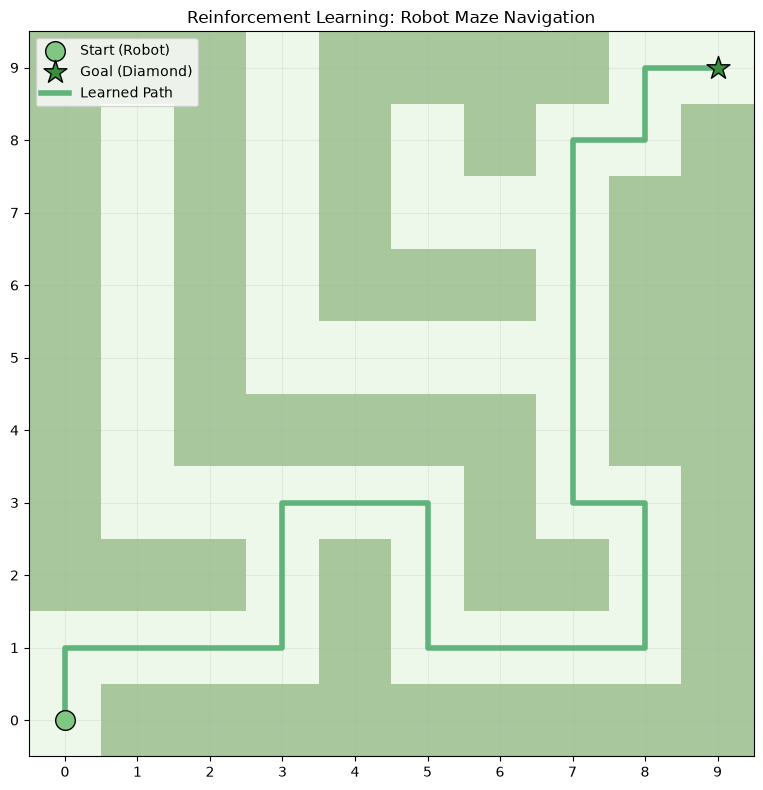
\includegraphics[width=0.86\textwidth,height=0.63\textheight,keepaspectratio]{images/q_learning_maze.png}
\caption{Mê cung và đường đi Q-learning từ output notebook.}
\end{figure}
\clearpage

\section{Bước 7: Hiển thị phần thưởng qua các episode}
Đồ thị dùng tổng phần thưởng của từng episode. Giai đoạn đầu chủ yếu nhận thưởng âm; về sau xuất hiện nhiều lượt có thưởng cao hơn nhưng vẫn dao động do agent còn thử hành động mới. Ảnh bên dưới là output gốc đã lưu trong notebook.

\begin{Code}
def plot_rewards(rewards):
    plt.figure(figsize=(10, 5))
    plt.plot(rewards)
    plt.title('Total Rewards per Episode')
    plt.xlabel('Episode')
    plt.ylabel('Total Reward')
    plt.grid(True)
    plt.show()


plot_rewards(rewards_all_episodes)
\end{Code}
\begin{figure}[H]
\centering
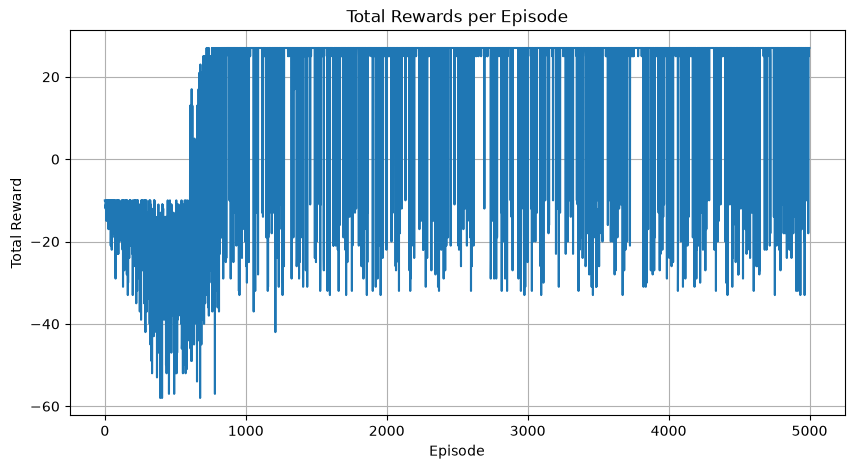
\includegraphics[width=0.86\textwidth,height=0.63\textheight,keepaspectratio]{images/q_learning_rewards.png}
\caption{Tổng phần thưởng theo episode từ output notebook.}
\end{figure}

\clearpage
\begin{thebibliography}{9}
\bibitem{google} Google Cloud, ``What is an AI agent? Definition, examples, and types,''
\url{https://cloud.google.com/discover/what-are-ai-agents}. Truy cập ngày 23/10/2026.
\bibitem{ibm} A. Gutowska, IBM Think, ``What Are AI Agents?,''
\url{https://www.ibm.com/think/topics/ai-agents}. Truy cập ngày 23/10/2026.
\bibitem{mckinsey} McKinsey \& Company, ``What is an AI agent?,'' 25/03/2025,
\url{https://www.mckinsey.com/featured-insights/mckinsey-explainers/what-is-an-ai-agent}.
Truy cập ngày 23/10/2026.
\bibitem{notebook} Phan Văn Khôi, \emph{reinforcement\_learning.ipynb},
\url{https://github.com/KhoiF/PTHTTM}, notebook tại
\path{src/Agent 01/reinforcement_learning.ipynb} và output lưu trong project.
\end{thebibliography}
\end{document}
